\section{Scomposizione in sottosistemi}
\justifying
A livello di funzionalità è possibile individuare tre grandi categorie, che le raggruppano in base ai tipi di utenti; è necessario precisare che queste categorie non sono mutuamente
esclusive (ad esempio la ricerca degli utenti può essere effettuata da chiunque):
\begin{itemize}
 \item Le funzionalità accessibili dagli ospiti: ricerca degli utenti, registrazione, login
 \item Le funzionalità accessibili dagli utenti registrati: ricerca, gestione del profilo, richiesta/accettazione di amicizie, invio di messaggi, invio di feedback, richiesta di
 nuove abilità
 \item Le funzionalità accessibili dagli amministratori: ricerca, gestione del profilo, richiesta/accetazione di amicizie, invio di messaggi, invio di feedback, gestione del set di
 abilità di sistema
\end{itemize}

\noindent
Tutte queste categorie si appoggiano ad un altro sottosistema, che è il database, il quale funge da archivio dei dati persistenti (vedi la sezione sul DB); infine come ultimo gruppo
si può identificare l'insieme di funzionalità volte a garantire e a disciplinare l'accesso al sistema a seconda del proprio status: la registrazione ed il login. Appare evidente una
parziale intersezione tra quest'ultimo sottosistema e quello delle funzionalità accessibili dagli ospiti: per essere più chiari possiamo considerare registrazione e login lato client
come parte del sottosistema dell'ospite, mentre gli stessi lato server come parte del sistema controllo.
\\
Il grafico nella prossima pagina mostra quello che ho appena scritto:
\pagebreak
\center
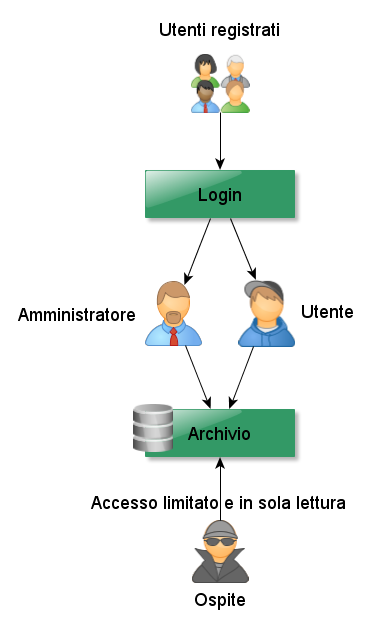
\includegraphics[scale=0.6]{sottosistemi.png}
\\
\noindent
\justifying
Il fatto che il grafo non sia orientato indica che ci sono interazioni in entrambi i versi degli archi.